We, the student council are a bunch of students, spread through varying terms and also members of diffrent faculties (physics \& astronomy and Mathematics \& computer science), which identfies as democratic, independent representants of physic"=, mathematic"=, and computerscience students. Accordingly students of both faculties are welcome, can make use of their voting right and their right to speak. Over the next sites you will find more specific things on how our student council works.

Furthermore every student of mathematics, physics or computer science is part of the "student council". If you enroll you are technically part of the student council, even though you are not activly participating. You have the right to make decisions, go and use it.

To enlarge the efficency of our student council we chose to split the subjects mathematics, physics and computersciencs content-wise, but organisation and events are held together. Thats why start with a common meeting and divide into two seperate meetings afterwards. These meetings are the key point of our work combined, everything important will be discussed in there. 

\begin{center}
\large
\textbf{Council Meetings}

\textbf{every Wednesday at 6 P.M. \gls{c.t.}}
\end{center}

\sidebar{
  \centering
  \chaptersidebarpushdown
  \ifthenelse{\boolean{druckversion}}{
        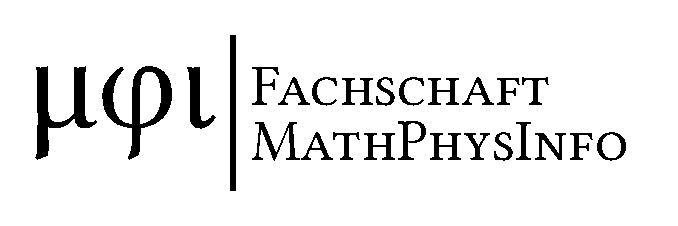
\includegraphics[width=3cm]{fs-logo_bw.pdf}
    }{
        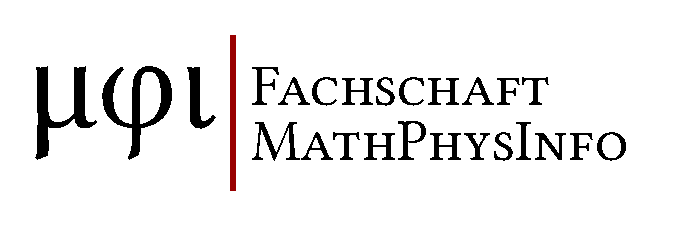
\includegraphics[width=3cm]{fs-logo_4c.pdf}
    }
}

\subsection{Change happens, if you make it happen\dots}
As already mentioned, we think about ourself as student representation. To achieve this it is especially important that we improve the subjects we study. We also we sometimes participate in political questions at our university. All of that is happening in a lot of diffrent ways.

At the begin of the lecture time you will sometimes get scripts handed out. We print these if the lecturers prepare one, for the most lectures since 2008 we pay them from so called "quality assurance funds". If you miss the lecture where the scripts are handed out, just come to the student council room and ask for them.

During the lecture time we actively work in commitees of the faculty, where we try to represent the students interst as much as possible. In the studycommitees exam regulations, enrolment regulations and generally everything connected to teaching and lecturing as a whole is discussed. For example they think about the concept of a bachelors course, so it is importantant for us to get ourselves a clear opinion in our own meetings and later on represent it in the commitees. In one commitee, which is in charge of processing the applies of diffrent professors and great lecturers with exciting lectures so they can work at the University of Heidelberg. After some preparation done by the commitee the members of the faculty board discuss and decide as commitees for the whole faculty. The six / eight student representatives in the faculty boards are elected annualy by the entirety of the students and are part of the student council. We also work out and discuss propositions and university-wide Finance"=, and positionpapers of the \gls{StuRa}.

At the end of the term you will most likely get to know one of our services: you can borrow old exams or reports of oral exams. Although we already got a quite big collection we are always happy about new reports. Especially for master lectures the stock is not that big. Thats why we appeal to you: bring your exams to the student council room and write new reports, because you also profitedstock is not that big. Thats why we appeal to you: bring your exams to the student council room and write new reports, because you also profited.

\subsection{I would rather go dancing\dots}
To clear up some persistent stereotypes about physicists, computer scientists and mathematicians ( and of course to have some fun ) we organise once in a term the legendary MathPhysTheo party and a few games nights. For a long time we organized the legendary "MathPhysRom". But since 2011 we got divine assitance by the student council of the theologists. New Name - still legendary: Come around, dance, party and \dots come to help us! We are always in search for volunteers in every possible departments. As a little present for helping you get a awesome tshirt, drinks- & wardrobe coupons of course free entrance! Dont worry: even though you are helping as a volunteer you still got enough time to party. 

If that is not enough for you, you can still come over at our room in INF 205, floor 1, room 01.301. At the Philosophenweg (physics) there also is a small cafe. Its an old garden cottage over at Philosophenweg 12 which was lovely renovated in summer 2009 and was usable 2013 again. You will find some sofas and tables, but also a coffee machine, water boiler and some cups. Coffee and tea are sold at cost price and sometimes there are cookies or 
sweets. At the moment its rarely openend but on tuesday for the \gls{StuRa} meetings most likely someone is there.

If you want even more information or struggeled to understand something you can just come around and ask. But if want to do something even better you can join one of our student council meetings. Thats where all the groups and commitees unite, topics are discussed and coordinated in here.

Once a lecture period we organize the \gls{FSWE}, which is a weekend somewhere deep in the near Odenwald. This weekend is dedicated to all relevant ttopics in student council work, which are discussed in smaller groups. Its also there to socialize and to have fun. Its for free for people who join us for the first time and the canteen could anticipate more than a little bit of our tasty food.
